\section{Method}
\label{sec:method}

We propose a discretization of the Laplace-Beltrami operator (LBO) that takes into account all geometric information that is given in Gaussian splatting and can serve as a quality measure for the surface information at the same time. 
As detailed in \cref{sub:bg:lbo}, the LBO encodes the local surface information so the main challenge is to construct the local neighborhood accurately, even though a collection of Gaussians has no explicit notion of connectivity. 
We explain how to do this in \cref{sub:method:graph}.
The second challenge is that most Gaussian splatting is optimized to render well and not as an accurate geometry representation. 
Methods like 2D Gaussians~\cite{Huang2DGS2024} or SuGaR~\cite{guedon2023sugar} aim to find a representation more localized on the surface but still contain many low-variance outliers. 
In \cref{sub:method:filter} we explain how the properties of the LBO can be used to determine if a geometrically converged representation was found and how to use this during training. 

\subsection{Local Neighborhood Construction}\label{sub:method:graph}

Gaussian splatting can be considered as a point cloud (the centers) with additional geometric information in form of a directional variance attached to each point. 
A straight-forward implementation of the LBO could just apply the point cloud Laplacian~\cite{sharp2020nonmanifold} to the center point cloud, however, this ignores valuable information that the variance gives. 
Instead of using the Euclidean neighborhood to estimate the local connectivity of the surface, we propose to use the Mahalanobis distance which can take into account the full Gaussian distribution present.

\paragraph{Mahalanobis Distance.} %
The Mahalanobis distance is a measure of the distance between a point and a distribution $\mathcal{G}$ with mean $\mu \in \mathbb{R}^d$ and covariance $\Sigma \in \mathbb{R}^{d \times d}$.
We only consider $d=3$ in this paper.
It is defined as
$$d_{M}(p, \mathcal{G})=\sqrt{(p-\mu)^T\Sigma^{-1}(p-\mu)}$$ 
for a point $p \in \mathbb{R}^d$.
See \cref{fig:mahalanobis} for a visualization.
Intuitively, Gaussian splats have a higher variance along the tangent directions of the surface, and a low variance in normal direction.
Thus, a neighborhood based on the Mahalanobis distance clusters together points that lie along side on the surface and give outliers a very high distance. 

However, we can only compute the distance between a \emph{point} and a distribution, but all elements of a Gaussian splatting are distributions. 
Computing the distance between two distributions, which is what we actually want, is possible, for example with the earth mover's distance but computationally very expensive. 
In practice, we approximate by taking a symmetric approach and building neighborhoods between splats where edge points are both their respective Mahalanobis neighbors.

\begin{figure}
    \centering
    (a) 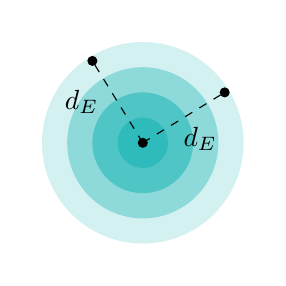
\begin{tikzpicture}[scale=0.8]
    \coordinate (A) at (0,0);
    \coordinate (B) at (1.3,0.8);
    \coordinate (C) at (-0.8,1.3);

    \foreach\i in {0.2,0.4,...,1} {
        \fill[opacity=\i,BlueGreen,rotate around={30:(A)}] (A) ellipse ({2-2*\i} and {2-2*\i});         
      }

    \draw[dashed] (A) -- (B) node [pos=.7, label=below:$d_E$] {};
    \draw[dashed] (A) -- (C) node [pos=.5, label=left:$d_E$] {};

    \draw[fill=black, draw=black] (A) circle (2pt);
    \draw[fill=black, draw=black] (B) circle (2pt);
    \draw[fill=black, draw=black] (C) circle (2pt);
\end{tikzpicture}%
 \quad (b) 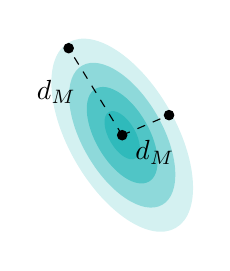
\begin{tikzpicture}[scale=0.85]
    \coordinate (A) at (0,0);
    \coordinate (B) at (0.7,0.3);
    \coordinate (C) at (-0.8,1.3);

    \foreach\i in {0.2,0.4,...,1} {
        \fill[opacity=\i,BlueGreen,rotate around={30:(A)}] (A) ellipse ({1-\i} and {2-2*\i});         
      }

    \draw[dashed] (A) -- (B) node [pos=.7, label=below:$d_M$] {};
    \draw[dashed] (A) -- (C) node [pos=.5, label=left:$d_M$] {};

    \draw[fill=black, draw=black] (A) circle (2pt);
    \draw[fill=black, draw=black] (B) circle (2pt);
    \draw[fill=black, draw=black] (C) circle (2pt);
\end{tikzpicture}

    \caption{Difference between the (a) Euclidean distance and (b) Mahalanobis distance. In (a) and (b) the marked points both have the same distance to the center, however, in the Euclidean and Mahalanobis distances, respectively. The Mahalanobis distance allows weighting directions differently, which we do in our methods using the variance of the Gaussians. }
    \label{fig:mahalanobis}
\end{figure}

\paragraph{Gaussian Laplacian.} 
The point cloud Laplacian requires a neighborhood $\mathcal{N}_v$ of $k$ nearest neighbors to be defined for each vertex $v$ which is then used to approximate the local surface. 
Instead of computing the Euclidean nearest neighbors, we compute the following for each Gaussian center:
$(p_i, p_j)$ is an edge if $p_i$ lies in the neighborhood of $p_j$, and $p_j$ lies in the neighborhood of $p_i$ using the $k$-nearest Mahalanobis neighbors. 
There can be multiple connected components in the constructed graph due to the existence of noisy Gaussian splats inside the objects. 
To filter out the Gaussian splats that do not align to the surface, we take the largest connected component to be the final graph representation of the object. %

The Laplacian of the Gaussian splatting is computed in the same fashion as for the point cloud Laplacian~\cite{sharp2020nonmanifold}. The point cloud is taken from the vertices of the constructed graph. Instead of computing the Euclidean distance, we construct the $k$ nearest neighbors in Mahalanobis distance. 
Additionally, the point normal estimation can be done by setting the normal of the point to be the the eigenvector corresponding to the smallest eigenvalue of covariance matrix of its Gaussian distribution instead of estimating the normals from the coordinates of the neighborhood. 
This set-up is applicable under the assumption that the 3D Gaussian splats are mostly flat and well aligned to the surface, which is achieved by previous methods such as SuGaR~\cite{guedon2023sugar} and GOF~\cite{yu2024gaussian}. As GOF is the SOTA approach to reconstruct the mesh with good geometry from 3D Gaussian splattings, we use GOF to train the 3D Gaussian splatting.  %

\subsection{Gaussian filtering} \label{sub:method:filter}

The optimization of a set of Gaussian splats often leads to outliers that do not contribute to the geometry or rendering. 
The original Gaussian splatting~\cite{kerbl3Dgaussians} already proposed to regularly remove splats with near zero opacity due to their low information.
When rendering a closed surface, splats on the inside will not be visible and thus can also take high variance forms without adding to the solution (but also not degrading it) but adding noise to the geometric information. 
We propose to use the same symmetric Mahalanobis neighborhood construction to filter out these noisy Gaussians by pruning splats that are not in the largest connected component.
See \cref{fig:filtering} for a visualization of the effect of filtering. 

\begin{figure}
    \centering
    \includegraphics[width=0.32\linewidth]{figures/cat0.png}
    \includegraphics[width=0.32\linewidth]{figures/cat0_filtered.png}
    \includegraphics[width=0.32\linewidth]{figures/cat0_adaptive.png}
    \caption{Example of the inside of the point cloud before(left), after (middle) filtering using the training from GOF~\cite{yu2024gaussian}, and using adaptive training (right).}
    \label{fig:filtering}
\end{figure}

\subsection{Adaptive Training} \label{sub:method:adaptive}
In previous work, the Chamfer distance~\cite{Huang2DGS2024,yu2024gaussian} is mainly used to evaluate the quality of geometry for Gaussian splatting. 
However, it is originally designed to evaluate the similarity between point clouds and thus does not take surface properties into account. 
To overcome this, we introduce the spectrum, i.e. the eigenvalues, of the Laplace-Beltrami operator as an evaluation metric. 
The eigenvalues are a global description of the geometry of a shape~\cite{REUTER2006shapedna} and can even be used to some extent to recover its geometry ("hearing the shape of a drum")~\cite{cosmos2019isospec}.
Although the ground truth spectrum of the reconstructed shape is unknown, we can use the eigenvalues to check for convergence of geometric properties, in addition to PSNR that is commonly used in 3D Gaussian splatting training.
Finally, the number of zero eigenvalues describes how many disconnected components an object has.
Removing all except the $k$ biggest disconnected components is an efficient tool to get rid of outliers when doing training. 
